%% myFigures.tex
% A common file to store all figure definitions
%
% In preparing your thesis, one of the first things you should do is
% organize your figures.  Then, one of the last things you'll do is
% reorder your figures so they display where you want them to in the
% text.  Organizing figure definitions in a common files helps:
%
%   1. Write new figures using earlier examples.
%
%   2.  Isolate code and minimize the risk of introducing bugs in the
%   final editing process.  Trust me, moving around just one line of
%   code is easier.
%
%   3.  Reuse figures in other papers.  <=== the best reason!
%
% Note command names can not include numbers and special characters.
%
% To make the file more searchable, use naming conventions that map
% the graphics filename labSetup.jpg to the command name \figlabSetup to the
% figure label fig:labSetup.
% 

\newcommand{\figproactiveFaultManagement}{\begin{figure}[H]
 \begin{center}
    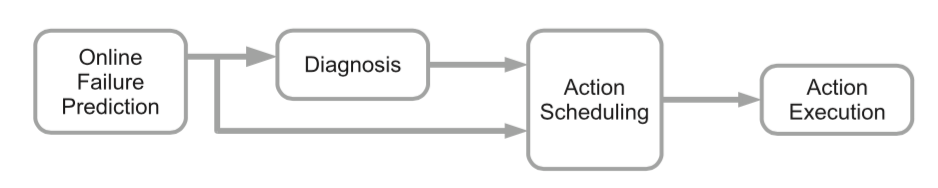
\includegraphics[width=6in]{proactiveFaultManagement}
     \caption[Proactive Fault Management~\cite{salfnerSurvey}]{The four stages of proactive fault management and how they integrate~\cite{salfnerSurvey}.}
     \label{fig:proactiveFaultManagement}
 \end{center}
\end{figure}
}

\newcommand{\figonlinePrediction}{\begin{figure}[H]
 \begin{center}
    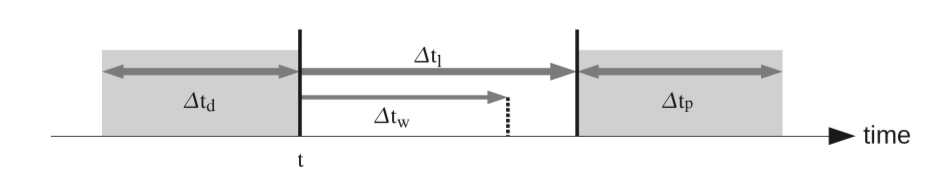
\includegraphics[width=6in]{onlinePrediction}
     \caption[Online Failure Prediction~\cite{salfnerSurvey}]{The timeline for OFP~\cite{salfnerSurvey}.}
     \label{fig:onlinePrediction}
 \end{center}
\end{figure}
}

\newcommand{\figfailureFlowDiagram}{\begin{figure}[H]
 \begin{center}
    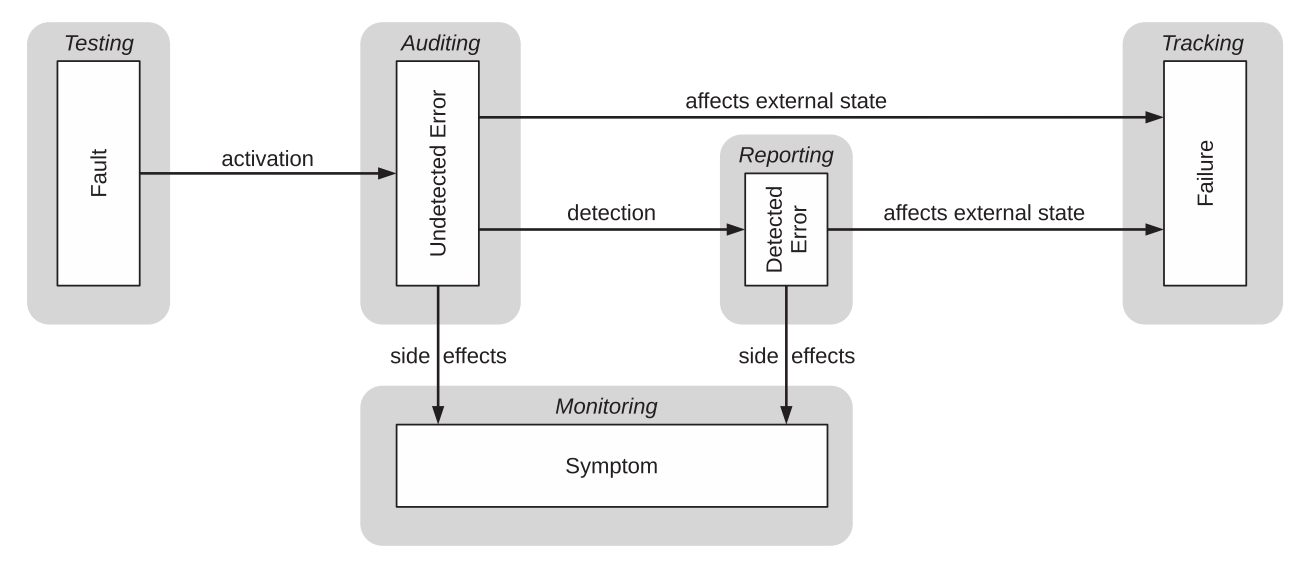
\includegraphics[width=6in]{failureFlowDiagram}
     \caption[Failure Flow Diagram~\cite{salfnerSurvey}]{How faults and errors evolve into failure with the associated methods for detection represented by enclosing gray boxes~\cite{salfnerSurvey}.}
     \label{fig:failureFlowDiagram}
 \end{center}
 %\vspace{-0.2 in}
\end{figure}
}

\newcommand{\figROC}{\begin{figure}[H]
 \begin{center}
    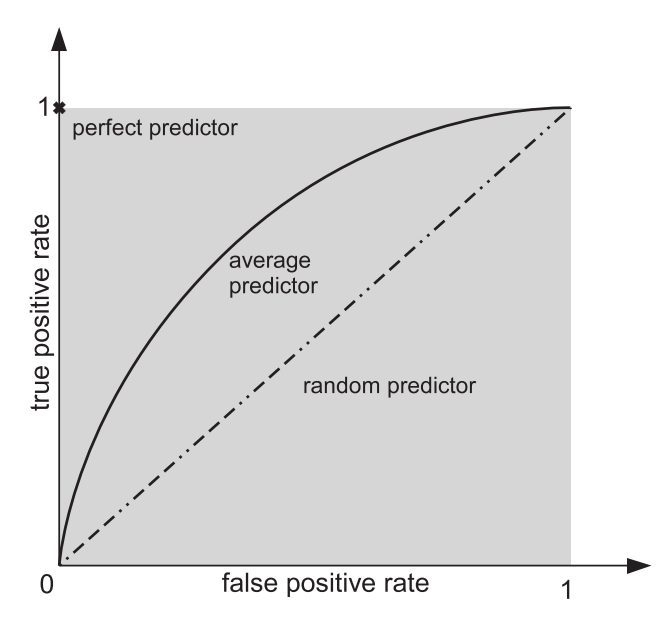
\includegraphics[width=3in]{ROC}
     \caption[Sample ROC Plots~\cite{salfnerSurvey}]{ROC plots of perfect, average, and random predictors~\cite{salfnerSurvey}.}
     \label{fig:ROC}
 \end{center}
\end{figure}
}

\newcommand{\figprecisionRecallCurve}{\begin{figure}[H]
 \begin{center}
    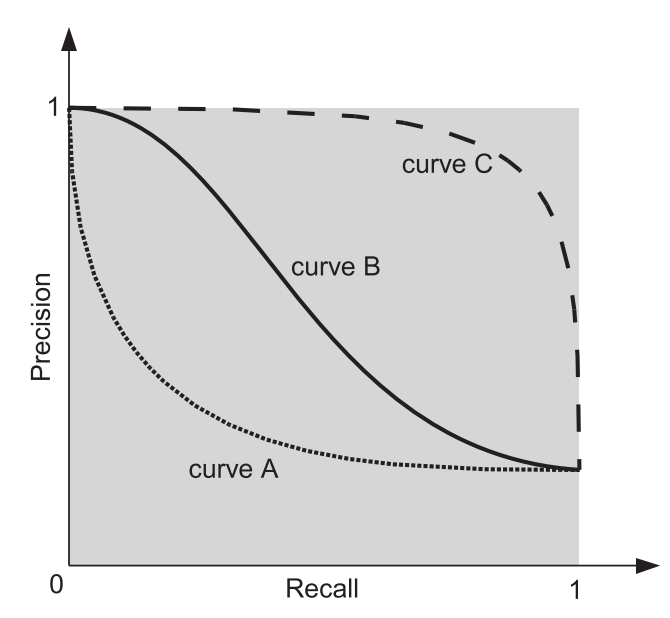
\includegraphics[width=3in]{precisionRecallCurve}
     \caption[Sample Precision/Recall Curves~\cite{salfnerSurvey}]{Sample precision/recall curves~\cite{salfnerSurvey}.  Curve $A$ represents a poorly performing predictor, curve $B$ represents an average predictor, and curve $C$ represents an exceptional predictor.}
     \label{fig:precisionRecallCurve}
 \end{center}
\end{figure}
}

\newcommand{\figpatternRecognition}{\begin{figure}[H]
 \begin{center}
    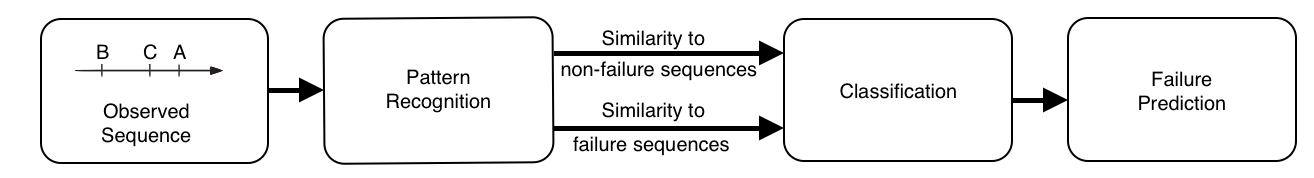
\includegraphics[width=6in]{patternRecognition}
     \caption[Pattern recognition in reported errors~\cite{salfnerSurvey}]{How pattern recognition is accomplished in reported errors~\cite{salfnerSurvey}.}
     \label{fig:patternRecognition}
 \end{center}
\end{figure}
}

\newcommand{\figAFP}{\begin{figure}[H]
 \begin{center}
    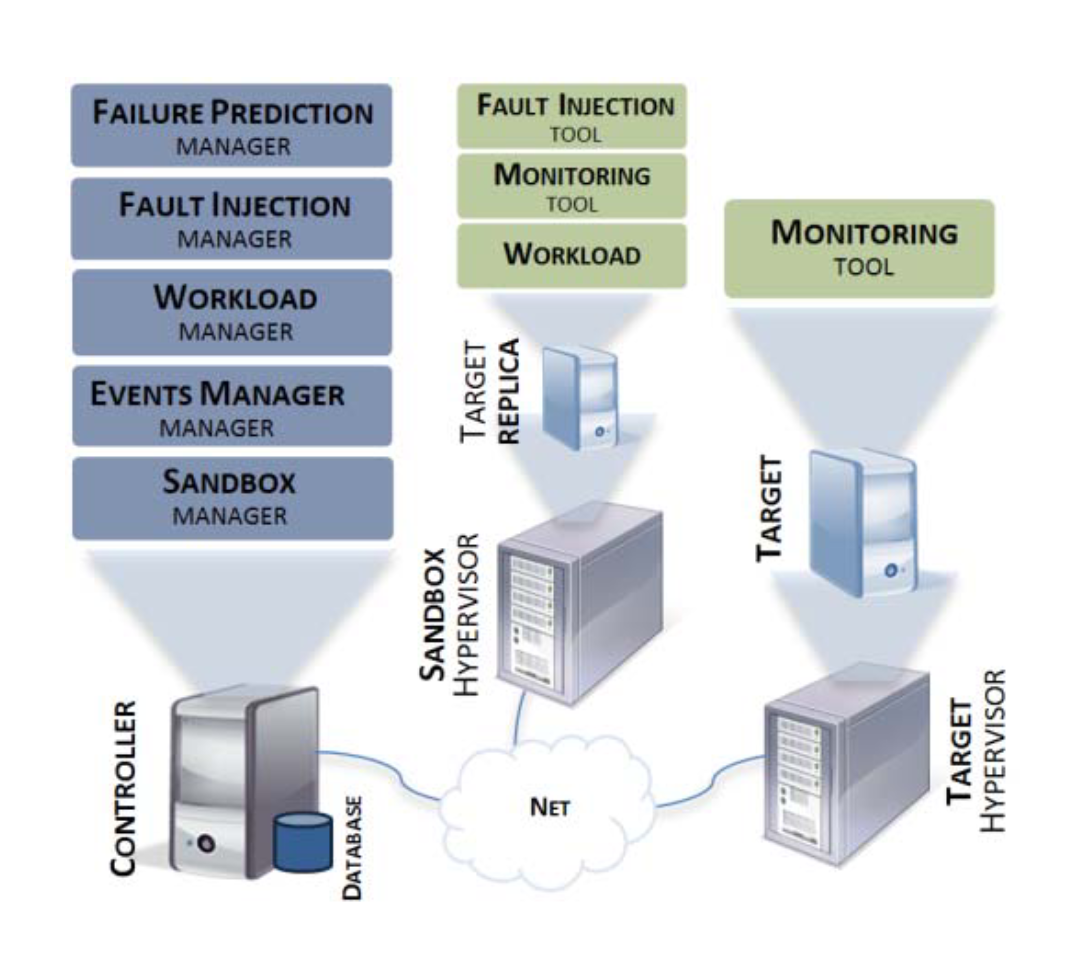
\includegraphics[width=5in]{AFP}
     \caption[AFP Framework Implementation~\cite{irrera2015}]{How the AFP framework is implemented~\cite{irrera2015}.}
     \label{fig:AFP}
 \end{center}
\end{figure}
}

\definecolor{airforceblue}{rgb}{0.36, 0.54, 0.66}
\definecolor{armygreen}{rgb}{0.29, 0.33, 0.13}

\newcommand{\figannotatedAFP}{\begin{figure}[H]
 \begin{center}
     \begin{overpic}[width=5in,scale=.25]{annotatedAFP}
       \put(8,0){
         \begin{tikzpicture}
           [node font=\footnotesize, label/.style={rectangle, draw,
           fill=airforceblue, text width=2cm, text badly centered, minimum
           height=0.5cm, rounded corners}]

           \node[label] (FPMgr)
             {\textcolor{white}{\ref{sec:failurePrediction}}};
           \node[label, below=1.2cm of FPMgr] (FIMgr) 
             {\textcolor{white}{\ref{sec:faultInjectionMgr}}};
           \node[label, below=1.3cm of FIMgr] (WMgr) 
             {\textcolor{white}{\ref{sec:workloadMgr}}};
           \node[label, below=1.2cm of WMgr] (EMMgr) 
             {\textcolor{white}{\ref{sec:eventsManagerMgr}}};
           \node[label, below=1.2cm of EMMgr] (SMgr) 
             {\textcolor{white}{\ref{sec:sandboxMgr}}};
           \node[label, below=4.75cm of SMgr] (Controller) 
             {\textcolor{white}{\ref{sec:controller}}};
         \end{tikzpicture}
       }

       \put(40,60.5){
         \begin{tikzpicture}
           [node font=\footnotesize, label/.style={rectangle, draw,
           fill=armygreen, text width=2cm, text badly centered, minimum
           height=0.5cm, rounded corners}]

           \node[label] (Sandbox)
             {\textcolor{white}{\ref{sec:sandbox}}};
           \node[label, below=1.2cm of Sandbox] (SBFITool)
             {\textcolor{white}{\ref{sec:faultInjectionTool}}};
           \node[label, below=0.95cm of SBFITool] (SBMTool) 
             {\textcolor{white}{\ref{sec:sandboxMonitoringTool}}};
           \node[label, below=0.95cm of SBMTool] (SBWorkload) 
             {\textcolor{white}{\ref{sec:sandboxWorkload}}};
         \end{tikzpicture}
       }

       \put(66,0){
         \begin{tikzpicture}
           [node font=\footnotesize, label/.style={rectangle, draw,
           fill=armygreen, text width=2cm, text badly centered, minimum
           height=0.5cm, rounded corners}]

           \node[label] (MonTool)
             {\textcolor{white}{\ref{sec:targetMonitoringTool}}};
           \node[label, below=7.85cm of MonTool] (Target)
             {\textcolor{white}{\ref{sec:target}}};
         \end{tikzpicture}
       }
     \end{overpic}
     \caption[Annotated AFP Framework~\cite{irrera2015}]{How the AFP framework is implemented~\cite{irrera2015} with modified components highlighted and numbered for reference.}
     \label{fig:annotatedAFP}
 \end{center}
\end{figure}
}

\newcommand{\figExecutionPhase}{\begin{wrapfigure}{R}{0.5\textwidth}
  \begin{center}
    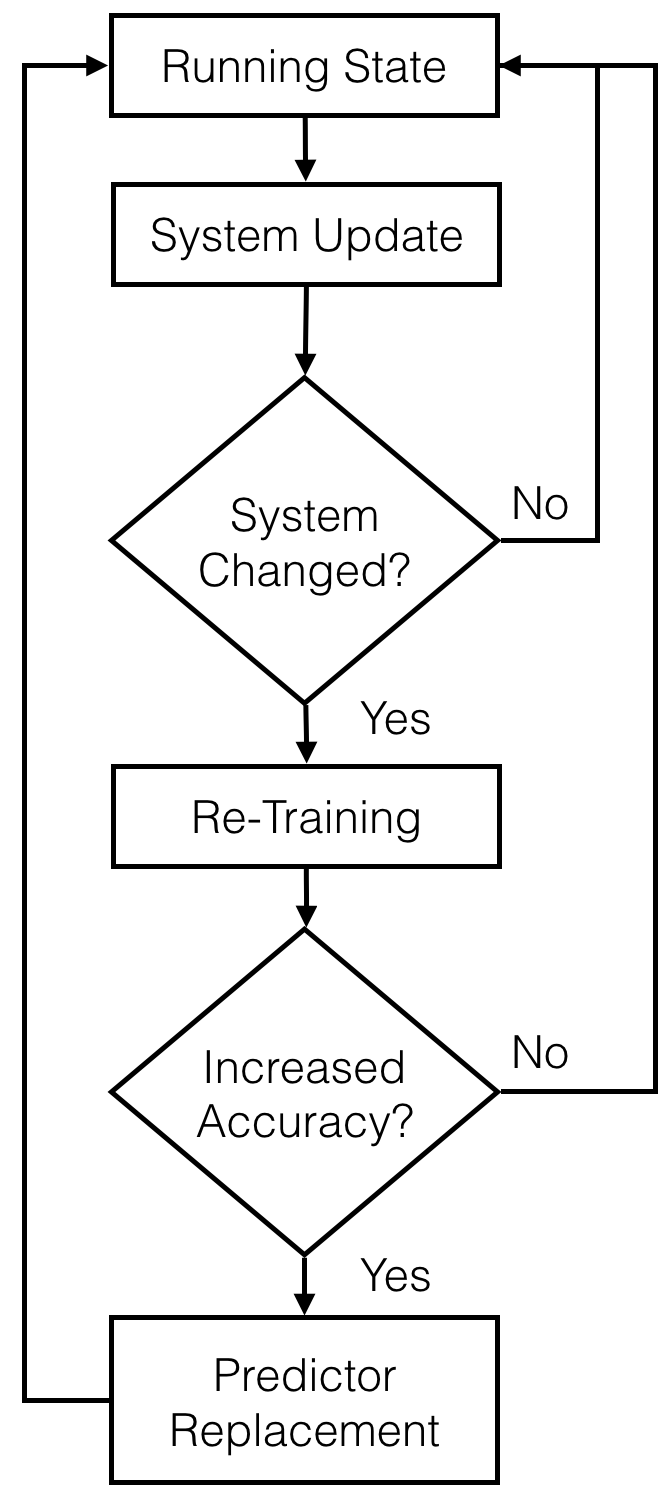
\includegraphics[width=2.5in]{ExecutionPhase}
    \caption[AFP Execution Phase~\cite{irrera2015}]{The flow of the major steps
    involved in the AFP framework execution phase~\cite{irrera2015}.}
    \label{fig:AFPFlow}
  \end{center}
\end{wrapfigure}
}

\newcommand{\figAuthDCPPS}{\begin{figure}[H]
 \begin{center}
  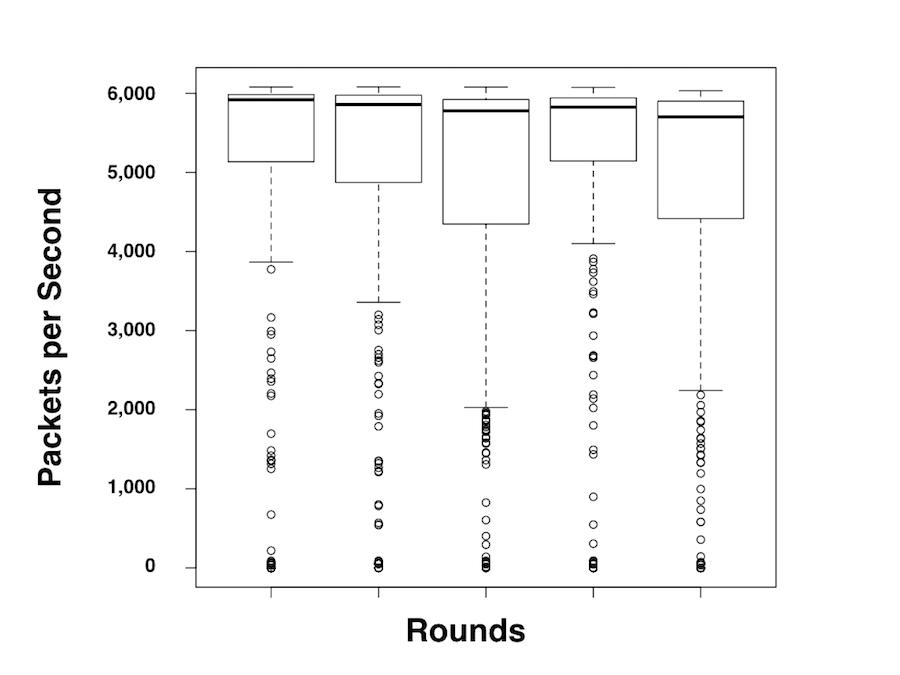
\includegraphics[width=4in]{authDCPPS}
  \caption[Domain Controller Packets per Second]{How many packets per second
  were sent or received by the domain controller across all five rounds of the
  first test.  In each test, we captured approximately 1.8 million packets.}
  \label{fig:authDCPPS}
 \end{center}
\end{figure}
}

\newcommand{\figAuthClientPPS}{\begin{figure}[H]
 \begin{center}
  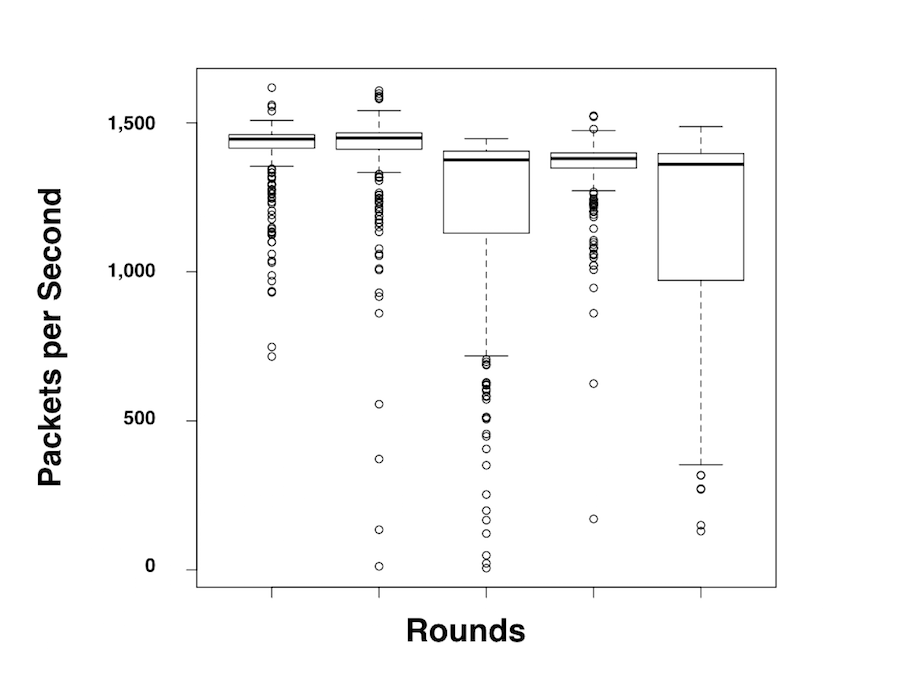
\includegraphics[width=4in]{authClientPPS}
  \caption[Client Packets per Second]{How many packets per second were sent or
  received by one of the clients across all five rounds of the first test.}
  \label{fig:authClientPPS}
 \end{center}
\end{figure}
}

\newcommand{\figAuthDCMetrics}{\begin{figure}[H]
 \begin{center}
  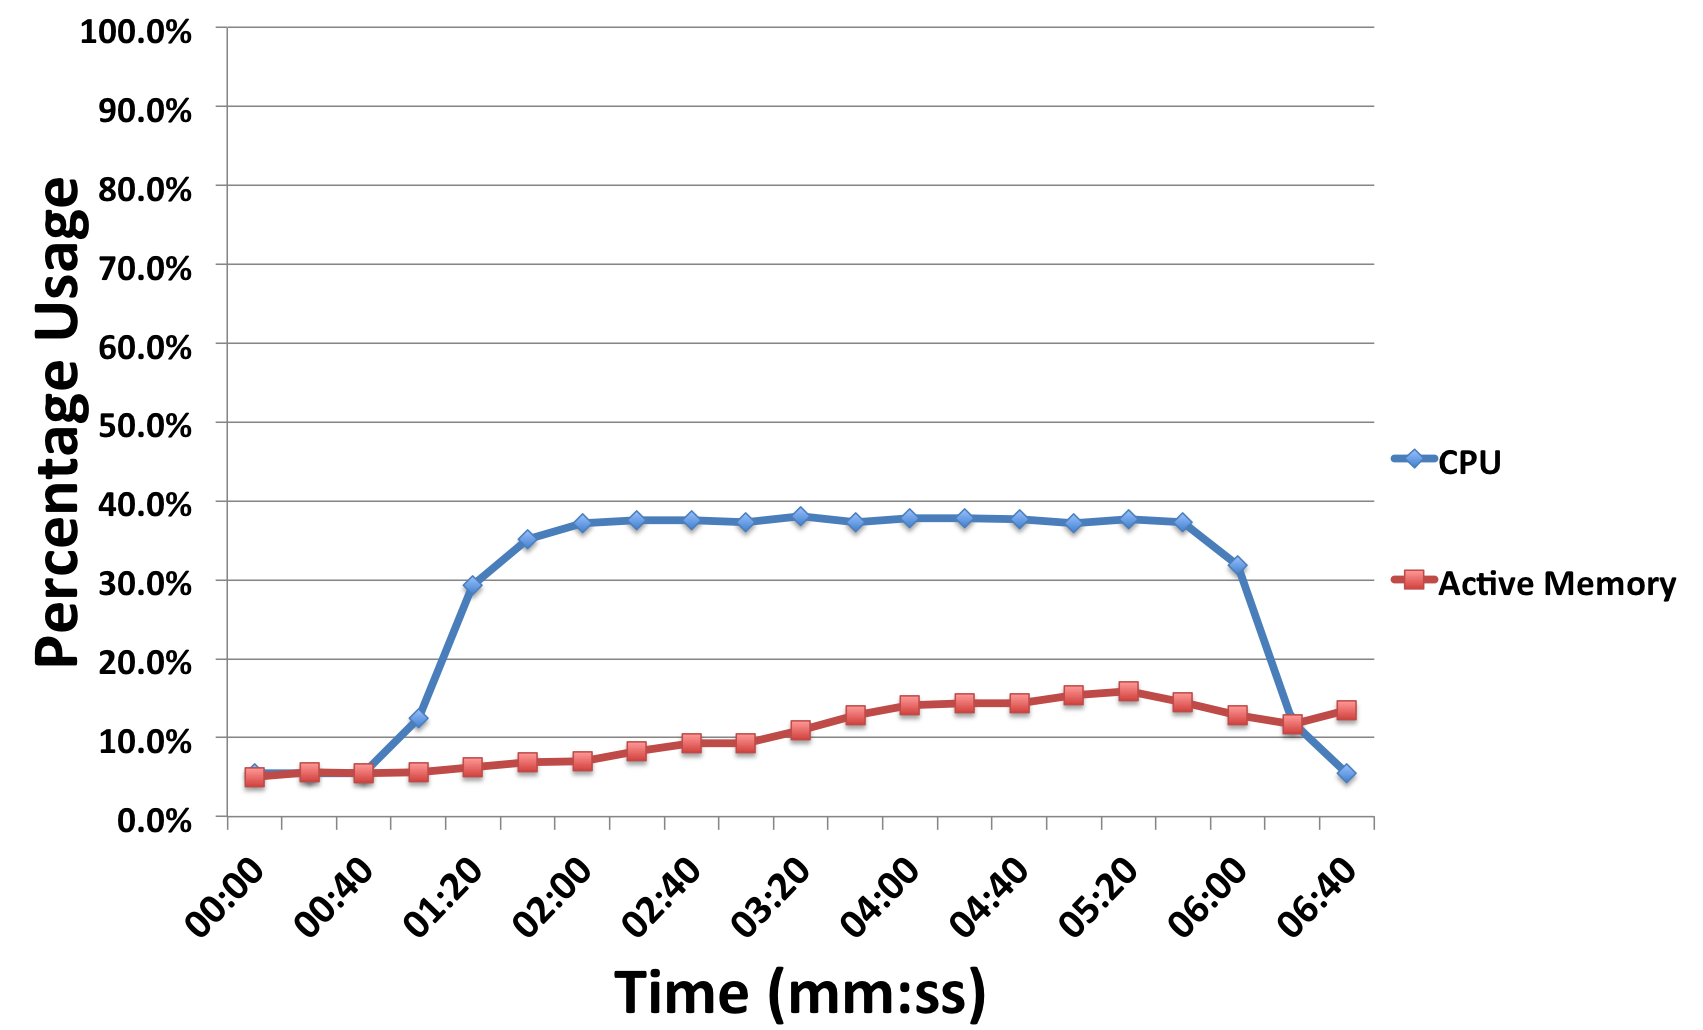
\includegraphics[width=4in]{authDCMetrics}
  \caption[Test 1:  Domain Controller Metrics]{Domain controller CPU and memory
  utilization during the first test.}
  \label{fig:authDCMetrics}
 \end{center}
\end{figure}
}

